
\subsection{Test Generation}

%\begin{algorithm}[!b]
\vspace*{3pt}
%\begin{algorithm}[ht]
\caption{Path Generation}\label{fig:pathAlgol}
\begin{algorithmic}[1]
{\footnotesize
\State \textbf{Inputs:} \textbf{ \textit{slices[]}} \Comment{\textit{The slices
array contains all of the slices
that are generated by the analyzing changes made to the modified version of the application.}}
\State \textbf{Outputs:} \textbf{\textit{paths}} \Comment{\textit{An array of all of the linearly
independent paths produced from the set of slices.}} 
\State \textbf{Declare:} \textbf{\textit{edges}} \Comment{\textit{A set of edges traveled by the path 
generator}}
\State \textbf{\textit{currentPath}} \Comment {\textit{A placeholder for the path currently being
generator}}
\Procedure{PathGeneration}{$slices$}
	\State $paths \gets \emptyset$ 
	\State $edges \gets \emptyset$ 
	\For{$n \longleftarrow 0 $, $n < slices$.size(), $n$++}
	\While{$slices[n]$.size()$ > 0$}
		\State $currentNode \gets slice[n]$.firstNode()
	    \State $currentPath \gets \emptyset$ 
	    \State $currentPath$.add($currentNode$)
	    \State PDGTraverser($currentPath$, $paths$, $edges$, $slice[n]$, $currentNode$) 
	\EndWhile\label{mainPathWhile}
	\EndFor
	\State ResolvePaths();
	\State \textbf{return} $paths$
	\EndProcedure
}
\end{algorithmic}
\end{algorithm}

%%\begin{algorithm}[htb]
\begin{algorithm}[ht]
\caption{PDG Traverser}
\label{fig:walkpath}
\begin{algorithmic}[1]
{\footnotesize
\Procedure{PDGTraverser}{$currentPath$, $paths$, $edges$, $slice$, $currentNode$}
		
	\While{$currentPath$[lastNode].occursBefore($slice$.endNodes())}
		\If{$currentPath$.containsNoDiffNodes() $\wedge$ $currentPath$.cannotReachAdiffNode()}
		\State	\textbf{Return}
		\EndIf
		\If{$slice[n]$.contains($currentNode$)}
			\State $slice[n]$.remove($currentNode$)
		\EndIf
		\If{$currentPath$[lastNode].getExits.Size() $> 1$}	
			\For {$n \leftarrow currentPath$[lastNode].getExits.Size()-1,0,$n$--}
				\If {$currentNode$.exitEdge($n) \notin  edges$}
					\State $edges$.add($currentNode$.exitEdge($n$)
					\If {$n$ == 0}
						\State $curentNode \longleftarrow currentNode$.exit(n)
						\State $currentPath$.add($currentNode$);
						\State continue(2); \Comment{\textit{Go back to while loop}}
					\EndIf
					\State PDGTraverser($currentPath$.copy(), $paths$, $edges$, $slice$, $currentNode$.exit($n$))
				\Else
					\If{$currentNode$.exitEdge($n$) $\in currentPath$}
					\State $currentNode \longleftarrow$ findFirstNodeOutsideofLoop() 
					\EndIf
				\EndIf
					
			\EndFor 
		\Else
			\State $curentNode \longleftarrow currentNode$.exit(0)
			\State $currentPath$.add($currentNode$);
		\EndIf
	\EndWhile
	\If{$currentPath$[lastNode].isNotASliceEndNode()}
		\If {$currentPath$[lastNode].canReachASliceEndNode()}
			\State $currentPath$.findSliceEndNode();
		\Else
			\State \textbf{Return}
		\EndIf
	\EndIf
	\State $paths$.add($curentPath$)
\EndProcedure
}
%\vspace*{3pt}
\end{algorithmic}
\end{algorithm}

%
%In this phase, we need three steps:
%(1) test path generation, (2) input constraint collection
%and resolution, and (3) test execution.
%The following subsections describe each step in detail.
%  
%\vspace*{3pt}
%\subsubsection{Path Generation}
%
%The path generator creates linearly independent test paths 
%using the slices collected from the previous step.
%A {\em linearly independent path} is a path that includes 
%at least one edge that has not been traversed previously 
%(in a given set of paths under construction)~\cite{pressman}.
%
%Algorithms~\ref{fig:pathAlgol}
%show how to generate test paths using slices. The algorithm 
%is separated into two parts. The first part, 
%Algorithm~\ref{fig:pathAlgol}, iterates through and gathers 
%the nodes from the slice to use in the PDG traversing procedure. 
%The second part, Algorithm~\ref{fig:walkpath}, is the PDG 
%traverser which follows a subpath through the PDG using 
%the nodes in the slice as a guide. Algorithm~\ref{fig:pathAlgol} 
%begins by iterating through every remaining node in each slice.
%
%The PDG traverser (Algorithm~\ref{fig:walkpath}) begins 
%by analyzing a node in the PDG. If the node being 
%processed occurs after every node in the array of 
%remaining slice nodes (line 2), the PDG traverser checks 
%to see if the currently processed node can reach an end node 
%(a node where change propagation terminates) in the original 
%slice (lines 30 and 31). If the node can, it adds the path to 
%an end node of the current path (line 32). Otherwise, the path 
%is discarded (line 33).
%
%If the node that is being processed occurs
%before any of the end nodes in the slice, the node is 
%checked to see if it can reach the changed node (line 3). 
%If it cannot, the path is discarded.
%The PDG traverser then checks to see if a node is
%in the array of slice nodes. If it is, that
%node is removed from the array (lines 6 and 7).
%Every time the PDG traverser encounters a node with more than 
%one edge that has not been traversed, it creates a new subpath 
%that is a copy of itself for each of these edges and follows 
%them (lines 9-18). Once construction of the path has been 
%completed, the path is added to the path array (line 37).
%
%After subpath construction is finished, the first node 
%in a subpath is traced to an entry point for the program, 
%and the last node is traced to an exit point for the program 
%(line 16 of Algorithm~\ref{fig:pathAlgol}). 
%Algorithm~\ref{fig:pathAlgol} describes the basic construction 
%of these paths while omitting, for brevity, all special cases 
%that occur for cyclic graphs (loops and recursion).
%
%\subsubsection{Constraint Gathering and Resolution}
%
%Because the generated test paths contain only input parameters, not 
%actual input values, the input values need to be assigned to the 
%parameters to make test paths executable.
%The constraint collector collects constraints on input
%values needed to execute a particular program execution path.
%Its inputs are the outputs from the PDG generator and path
%generator. The top-level activities in the constraint collector
%are parsing the path and PDG XML files, generating constraints
%for each path, and writing the collected path constraints to
%an XML file. 
%
%Constraint collection begins with path nodes that contain
%a conditional statement. The primary activities to collect
%constraints are determining the truth value of conditional
%statements and reducing the conditional expression in these
%statements. 
%%A constraint is recorded only if it is not
%%a duplicate for a previously recorded constraint.
%A path constraint corresponds to a path PDG node with an
%``if'' statement. To determine the truth value of
%a constraint, the collector looks ahead one node in the
%path node list and examines the node type (which will be
%necessarily either \textit{true} or \textit{false}). After
%determining the constraint truth value, the constraint
%condition is then recursively reduced. Reduction of
%an expression involves parsing the expression string
%to determine the expression type (using regular expression
%matching), creating an expression object with this type,
%assigning any expression attributes from the parsed information
%(e.g., operator type) to the expression object, and generating
%appropriate expression objects for child expressions (if any).
%If there are child expressions, they are recursively reduced
%in the same way.
%
%Each type of expression provides its own method for reducing
%child expressions, in order to take advantage of information
%on the reduction context. For example, a compound boolean
%expression must have child expressions that are themselves
%boolean. When generating child expressions, this information
%can be provided, in addition to that which is provided by
%regular expression matching. This is useful in verifying
%that generated expressions are of the correct type.
%
%If regular expression matching determines an expression
%to be a variable (e.g., \$num\_of\_files), the reduction
%process involves additional steps:
%
%\begin{enumerate}
%  \item The collector backtracks in the path node list,
%starting at the index of the variable node. It continues
%backtracking until a PDG node is encountered that provides
%a definition of the variable, or until the beginning of
%the list is reached. In the case that a definition is found,
%the expression generated for the variable is of the complex
%variable type. This type is used for variables that can be
%defined in terms of other expressions. If, instead, no
%variable definition is found before reaching the start of
%the list, the expression generated is of the simple variable type.
%
%  \item Regular expression matching is performed on the
%variable expression string to determine if it is indexed
%(e.g., \$files[\$id]). These correspond to PHP array variables.
%An expression is then generated for the index of the array, and
%the generated expression for the variable is an indexed version
%of the type determined via backtracking (i.e., simple or complex 
%type).
%\end{enumerate}
%
%The recursive reduction process terminates on expressions of
%simple type, since simple type expressions do not contain
%child expressions that need to be reduced.
%After collecting a constraint, the collector records it for
%inclusion in the output. 
%%This step is only done if an equivalent
%%constraint is not already present in the list in order to
%%avoid outputting duplicate constraints. 
%Once all path constraints
%have been generated, the collector writes the constraint information
%in XML format. 
%
%The tool uses an existing constraint solver, {\em Choco},
%to determine the input values that satisfy the constraints
%for a given execution path (if such satisfaction is feasible).
%{\em Choco} is an open-source software and  consists of a set
%of libraries written in Java that provide many constraint solving
%features. It provides direct support for solving numeric and
%boolean constraints. We also use it to solve string constraints
%by mapping these constraints to equivalent constraints on integers. 
%Once all input values have been created, they are stored in XML file 
%format to be used later by the test execution engine.
%These files contain information about program paths and a list of input 
%variables for the paths. For each input variable, the variable type, 
%name, and value are given. 
%Resolving the inputs that use built-in PHP functions is not supported 
%by our tool, so those inputs require manual resolution. 
%Further, the constraint resolution tool sets the time limit for 
%input resolution, and it reports infeasible when it cannot find 
%the value within the time limit. Also, if the conditions for a 
%variable have conflict, the tool reports that case as infeasible.
%
%\subsubsection{Test Execution}
%
%Having assigned all input values to the parameters in the test 
%paths, we implemented a test execution engine that executes
%test cases over web applications using Selenium~\cite{selenium}.
%We used the Selenium WebDriver API (more specifically, the FirefoxDriver) 
%to set the web page elements according to the variable constraints for 
%the given execution path being tested. If test execution requires setup 
%logic, such as authentication, this is also performed using the WebDriver 
%API. Finally, the WebDriver API is used to execute the PHP file and the 
%results are passed to the test engine.
%As mentioned earlier, web elements are created manually becasue the current 
%path generator does not provide them.
%
%The reason that we have chosen to use the WebDriver API is that it allows us 
%to perform all the activities that will be required: finding and setting web 
%elements; performing any setup tasks required before the test case can be 
%executed (such as authentication); retrieving test execution results in the 
%HTML format.
%
%To give a better understanding of how the approach works, we use an e-commerce 
%example. Assume that we have two PHP files, login.php and add\_card.php, both 
%of which are accessed on different web pages. login.php contains the login 
%form that users can register/authenticate with, and add\_card.php allows 
%authenticated users to add their credit card information. Both login.php 
%and add\_card.php contain entry points for certain execution paths.
%
%If add\_card.php was modified between Version 1 and Version 2, we can run 
%the toolchain on this version pair and determine the constraints necessary 
%to test execution paths with entry points beginning in that file. Using 
%the Selenium WebDriver API, we can first access the login form contained 
%on login.php to register/authenticate the user. Afterwards, we use the 
%same API to directly execute add\_card.php, after initializing the values 
%of the web elements associated with path constraints. It would not be 
%necessary to start from login.php, since the PHP \$\_SESSION variables 
%used for authentication would still be valid during execution of add\_card.php, 
%regardless of the navigational path for arriving at this page. The results 
%of executing add\_card.php are recorded as an HTML file.
%
%
%
\subsection{An Example of Test Path and Input Generation}

\begin{figure*}[htb]
%\begin{figure*}[!b]
  \centering
  \begin{minipage}[t]{0.31\textwidth}
    \centering
    \lstset{language=PHP, title=v0.php (original version),
basicstyle=\footnotesize,  tabsize=2}
    \lstinputlisting{figures/v0.php}
  \end{minipage}
  \begin{minipage}[t]{0.31\textwidth}
   \lstset{language=PHP, title=v1.php (modified version),
basicstyle=\footnotesize, tabsize=2}
    \lstinputlisting{figures/v1.php}
  \end{minipage}
    \begin{minipage}[t]{0.35\textwidth}
      \caption*{\\PDG for v0 and v1}
      \vspace*{6pt}
    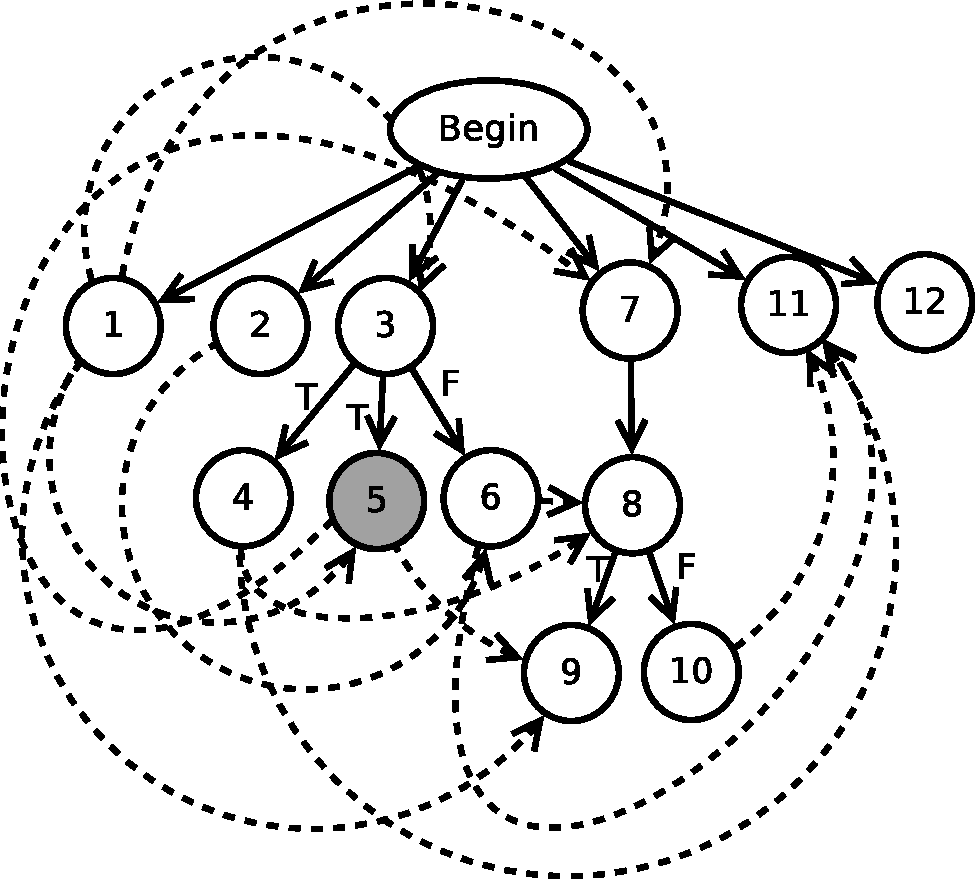
\includegraphics[width=\textwidth]{figures/flow2.pdf}

  \end{minipage}
  \caption{Path Generation Example Program}
%\vspace*{-5pt}
  \label{fig:example}
\end{figure*}



%We illustrate how we generate test paths using program slices.
%Suppose we have a simple PHP program (v0.php) and its 
%modified program (v1.php) as shown in Figure \ref{fig:example}.
%The rightmost graph shows a PDG for v0.php and v1.php.
%
%In the PDG, the solid lines represent control dependence edges, 
%and the dashed lines represent data dependence edges. 
%As the example shows, statement 5 has changed, so our slicing
%algorithm takes node 5 and variable $a$ ($<$5, $a>$) as a slicing 
%criterion. By performing forward and backward slicing, the slice 
%with respect to $<$5, $a>$ includes nodes 1, 5, 7, and 9 (node 1 
%from backward slicing, and nodes 7 and 9 from forward slicing). 
%
%Having obtained this slice, the path generator creates subpaths 
%starting from the first node in it (in this example, node 1). 
%As the tool walks the path using control flow information, 
%it adds nodes 2 and 3 to a subpath (\{1, 2, 3\}). 
%Once the path generator reaches node 3, it has a choice to 
%explore one of the control successors (4 and 6).
%When the tool analyzes the path containing edge 
%3 $\rightarrow$ 4, it sees that the next 
%control successor is node 5, yielding a subpath of 
%\{1, 2, 3, 4, 5\}. 
%When the tool analyzes the path containing edge 
%3 $\rightarrow$ 6, it discovers that
%there is no path from node 6 to node 5. It then discards
%path \{1, 2, 3, 6\}. 
% 
%Continuing with the remaining edges, the tool produces
%a subpath of \{1, 2, 3, 4, 5, 7, 8\}. Because node 8 
%is another branching node, the tool yields subpaths 
%\{1, 2, 3, 4, 5, 7, 8, 9\} and \{1, 2, 3, 4, 5, 7, 8, 10\}. 
%Edges 8 $\rightarrow$ 9 and 8 $\rightarrow$ 10 are marked as 
%covered by the path generator. The tool then recognizes that 
%subpath \{1, 2, 3, 4, 5, 7, 8, 10\} ends with a node that is 
%outside the impact set. (It is impossible to go from node 10 
%back to nodes \{1, 5, 7, 9\}.) The tool also recognizes that 
%there is no path from node 7 to node 9 that goes through node 10. 
%The tool then discards this path. This process is repeated until 
%all nodes in a slice have been visited.
%
%Having generated subpaths that contain all nodes in a slice,
%the tool walks the program dependence graph from the 
%first node to the beginning of the program (In this case, node 1 
%is at the beginning.) and walks the last node in the path to the 
%end of the program by adding nodes 11 and 12 to it.
%In this example, the tool generates one final path,
%\{1, 2, 3, 4, 5, 7, 8, 9, 11, 12\}.
%Note that, without applying our approach, we need to generate
%four linearly independent paths to test the modified program,
%v1.php. 
%
%The next step is to generate inputs for the created path. 
%First, the constraint collector gathers constraint information
%by analyzing all the path's branching nodes. 
%In our example for path \{1, 2, 3, 4, 5, 7, 8, 9, 11, 12\}, 
%three constraints are collected:  
%\$ POST[`inputA'] $<$ 12 , \$ POST[`inputA']-3 $>$ 7, and 
%\$ POST[`inputB'] $==$ 5. 
%Using a constraint solver, we can choose input values 11 and 
%5 for \$ POST[`inputA'] and \$ POST[`inputB'], respectively.
%Once these values are resolved, the test execution engine
%can simply use them as inputs for the web application to walk 
%the desired path.
%
% 

